% !TEXroot = ../thesis.tex

\chapter{Syntactic part} \label{sec:methodology}
Based on the Analytical part~\ref{sec:analytical} let us create  mathematical models to predict customer behavior which consist of
vendor, psychology and loyalty sub-models combined in Hidden markov model (HMM) to final prediction model called Customer behavior HMM.
We expect to get better results than by using prediction based on standard regression model methods (see section~\ref{sec:regression}) to predict customer behavior in e-commerce.
Finally, our approach will return future income for online store based on previous data with better aberration than linear or polynomial regression has.
Customer behavior HMM directly returns number of predicted orders used to calculate estimated income.
For successful prediction open data for store strength and customer satisfaction and some predefined and computed variables from store will be used.

\section{Customer behavior Hidden Markov Model} \label{sec:submodels}
Our model is based on Markov models (see section~\ref{markovmodel}) and consist of these three states: order, not finished order, no order decision.
Model simulates customer behavior during order process and tries to return the way with the most probability.
Then reads the results by Viterbi algorithm and checks if the order was made.
As inputs serves probabilities from predefined submodels used as transition matrix for HMM, number of customers in the predicted period,
probability matrix of initial states and average income per order from previous period.
On the figure~\ref{Model schema with interaction} the computation flow and interactions between models in Customer behavior HMM is presented.\\
\begin{figure}[h!]
    \begin{center}
        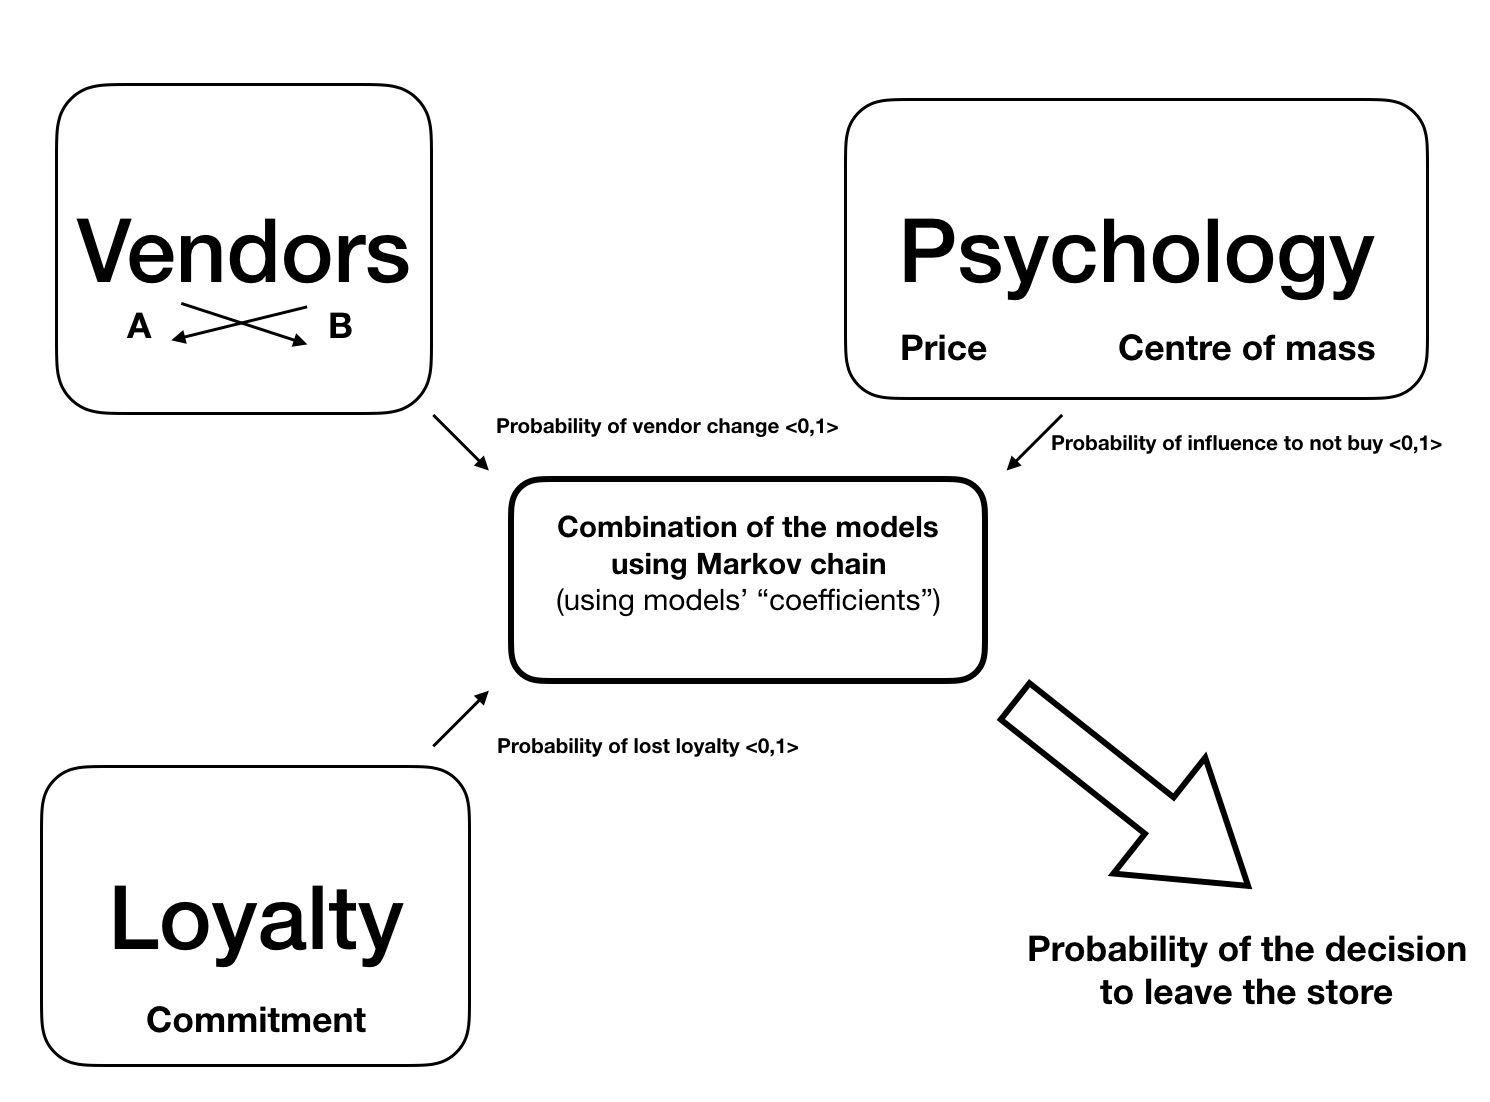
\includegraphics[width=100mm]{computation_schema.png}
    \end{center}
    \caption{Computation flow and interactions between models in Customer behavior HMM}
    \label{Model schema with interaction}
\end{figure}\\
Our specific situation which is different from standard HMM is described on the figure~\ref{states} and tells that our states are not connected together as usually in HMM.
This is caused by specific order processes which are not directly connected to each other (see flowchart~\ref{flowchart_overview}).
In the first step the model got predefined data from initial part (see section~\ref{sec:preprocessing}) and goes through the model according to the following steps:
\begin{enumerate}
    \item get probability from Vendor submodel (see section~\ref{subsec:model_vendors}),
    \item get probability from Psychology submodel (see section~\ref{subsec:model_psychology}),
    \item get probability from Loyalty submodel (see section~\ref{subsec:model_loyalty}),
    \item combine submodels data in Hidden Markov model (see section~\ref{subsec:combining_models}),
    \item read invisible states by Viterbi algorithm,
    \item check result matrix produced by Viterbi and save the number of success orders,
    \item calculate prediction income.
\end{enumerate}\\
\begin{figure}[h!]
    \begin{center}
        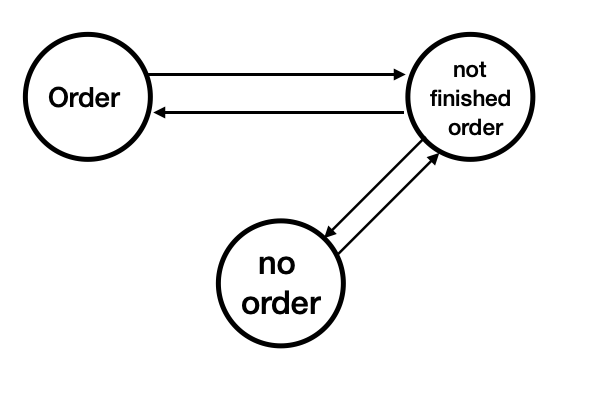
\includegraphics[width=80mm]{states.png}
    \end{center}
    \caption{Overview of states and their combinations}
    \label{states}
\end{figure}\\
\subsection{Vendors submodel} \label{subsec:model_vendors}
For simplification, we will take into account only two vendors market share, without 100\% domination, because on a real
market 100\% monopole is unlikely to see and then we will reflect only main competitor.
From that condition it is evident that for market to which vendor dominates it will return false positive results.
Our model is based on equations from Brands (section~\ref{eq:10}) and from those equations we will get probability of vendor
change from vendor $A$ to vendor $B$ and if the vendor $B$ will have more strength than vendor $A$, it will disrupt the
computation and customer will leave our store without completing buying process successfully.
Results of this computation will in form of probability for each iteration of buying process simulation in an interval $[0,1]$.
Data for this model will come from open data provided by google.com, heureka.cz/heureka.sk and national governments.
That data will be combined with calculated price indexes downloaded from shopycrm.com tool (see flowchart~\ref{flowchart_vendor}):
\\
\begin{equation} \label{eq:13}
V_{xy} = \beta H(P_x-P_y) + \gamma H(Qx-Qy) + \delta H(Px-Py)H(Q_x - Q_y),
\end{equation}
\\
where $\beta, \gamma, \delta$ are non-negative, $P$ is prices of vendors products, $Q$ is a quality index of vendor, $H$ is a Heaviside function which has values:\\
\begin{equation} \label{eq:14}
\begin{array}{l}
    H(s) = 1, s > 0 \\
    H (s) = 0, s \leq 0
\end{array}
\end{equation}
\\
\subsection{Psychology submodel} \label{subsec:model_psychology}
Psychology aspect is trying to simulate customer behavior in situations like a prices aspect, society influenced, mood aspect, actual needs and so on.
In this model we will simplify only price effect and center of mass effect.\\
\\
\textbf{Price aspect} \label{subsubsec:model_psychology_price} is described by equation:\\
\\
\begin{equation} \label{eq:15}
\overset{-}{Q} = \frac{1}{n_p} \sum_{i=1}^{n_p} Q_i,
\end{equation}
\\
where $Q_i$ number of orders for product $i$ per day divide amount of orders per same day, prom interval $[0,1]$, $n_p$ number of products in store:\\
\begin{equation} \label{eq:16}
\alpha_{ij} = \frac{C+max(Q_j, \overset{-}{Q})}{C+max(Q_i, \overset{-}{Q})}.
\end{equation}
\\
Coefficient C is used to be $\alpha_{ij}$ always positive.
\textbf{Center of mass aspect} \label{subsubsec:model_psychology_mass} is applied as a part of sociology to our psychology model.
Marketers use it for manipulating with customers in global way.
Like a black friday, Cyber monday etc., in that days stores manipulate with our psychology by discount prices:
\\
\begin{equation} \label{eq:17}
\overset{-}{P} = \frac{1}{n_p} \sum_{i=1}^{n_p} P_i,
\end{equation}
where $P_i$ is defined as product price minus retail recommend price divide average price, $n_p$ number of products in store:\\
\begin{equation} \label{eq:18}
\beta_{ij} = \frac{C+max(P_j, \overset{-}{P})}{C+max(P_i, \overset{-}{P})}.
\end{equation}
\\
This model returns final probability as count of $\alpha$ and $\beta$ probabilities for customer decision to make action from interval $[0,1]$.
\\
\subsection{Loyalty submodel} \label{subsec:model_loyalty}
This submodel is based on Luarn \& Lin research~\cite{luarn} and we changed their model for our needs:\\
\begin{equation} \label{eq:19}
L = \frac{R+Z}{Z},
\end{equation}
\\
where L is probability of whole loyalty model, R is probability of separate loyalty model, Z is probability of commitment model.
\\
As we see on figure~\ref{Loyalty scheme} Loyalty model consists of three sub-models (Trust, Customer Satisfaction, Perceived value)
but commitment model consist of only Trust and Customer Satisfaction.
Weight coefficient $a,b,c,d,e$ were used to combine Trust, Customer satisfaction and Perceived value (see flowchart~\ref{flowchart_psychology}).\\
\begin{figure}[h!]
    \begin{center}
        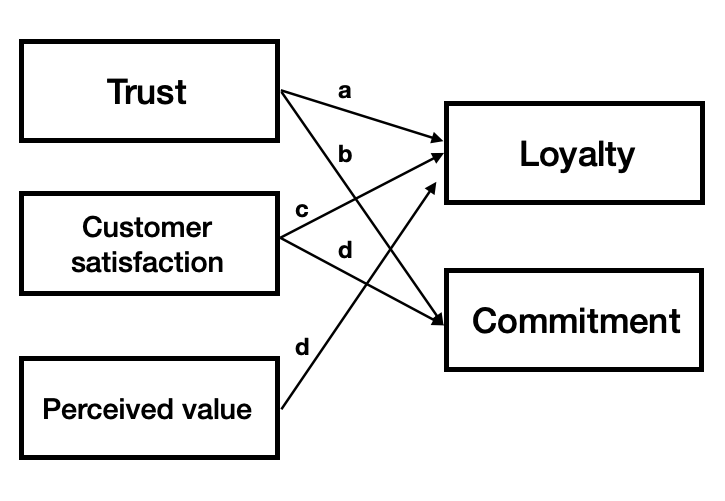
\includegraphics[width=100mm]{loyalty.png}
    \end{center}
    \caption{Computation flow for loyalty and commitment~\cite{luarn}}
    \label{Loyalty scheme}
\end{figure}\\
\\
\textbf{Trust} can be defined as:\\
\begin{equation} \label{eq:20}
T = \frac{1}{n} \sum_{i=1}^{n} O_i,
\end{equation}
\\
where $O_i$ is the number of orders divided by number of visitors per day $i$.
\\
\\
\textbf{Customer satisfaction} are datasets get from open data per each day, individual satisfaction.
For simplification of the situation we will use average satisfaction per whole store (see flowchart~\ref{flowchart_loyalty}).
\textbf{Perceived value} (see defined values in~\ref{perceived}) is subjective value, which depends on the strength of the store.
\subsubsection{Commitment and Loyalty} \label{subsubsec:model_loyalty_commitment}
\textbf{Commitment} is making the actual choice every day or other period basis to keep up with something e.g. a relationship, personal goal, a task, etc.
We would have to hold ourselves accountable to keep a commitment to something or someone.
Similarly, being loyal involves holding ourselves accountable as well.\\
Against of \textbf{Loyalty} which is usually seen as a character trait rather than a conscious decision.
This model returns probability for customer decision to not leave the store from interval $[0,1]$.\\
\subsection{Combining submodels to decision process} \label{subsec:combining_models}
As a combination method Hidden Markov Model (HMM) (see flowchart~\ref{flowchart_markov}) was selected.
All separate models return probabilities which were put together to square matrix used as input to HMM (see section~\ref{markovmodel}).
These probabilities will be combined with specific weights (coefficients) to always prevent positives results.
Let us create approach to store information from Customer behavior HMM about successful order prediction.
In the same way the model is able to predict when the customer leaves the store, but this situation was not added to our prediction experiment and should be used in future updates.
Then based on that prediction data, calculation of future income for store was done.
Our designed model consists of three sub-models, which are partially dependent on each other.
Vendor,\ psychology and loyalty models we created for our prediction to simulate customer behavior.
Then partial results were combined into complex prediction mechanism, as you can see on figure~\ref{Model schema with interaction}.
\\
HMM in combination with Viterbi algorithm will be used to detect hidden states, which will be reflected in predefined weights for specific
industries to return data matrix with prediction.
In a Hidden Markov Model (HMM), we have an invisible Markov chain (which we cannot observe), and each state
generates in random one out of $k$ observations, which are visible to us.
This final generated state is not important for us.
We need know the way true states.
This why Viterbi is used
Let’s look at our situation.
Suppose we have the Markov Chain from above, with three states (order, not finished order and no order decision),
$P$ - the transition probability matrix and $q$ — the initial probabilities.
This is the invisible Markov Chain — suppose we are not with the customer and can not see the decision.
We can, however, see the results from the customer, and suppose there are two possible observations: order and no order decision.\\
Customer behavior HMM is described by equation:\\
\\
\begin{equation} \label{eq:25}
P = \left(
\begin{pmatrix}
    V_{xy} & V_{xy} & V_{xy} \\
    \alpha + \beta & \alpha + \beta & \alpha + \beta \\
    \frac{R + Z}{Z} & \frac{R + Z}{Z} & \frac{R + Z}{Z}
\end{pmatrix}|
\begin{pmatrix}
    l & m & k \\
    l & m & k \\
    l & m & k
\end{pmatrix}
\right),
\end{equation}\\
\\
where $V_{xy}$ is vendor probability, $\alpha, \beta$ are partial results from psychology submodel, $R$ is partial
loyalty and $Z$ is commitment probability, and $l,m,k$ are coefficients of initial states probabilities.
